\documentclass{standalone}
\usepackage{tikz}
\usetikzlibrary{patterns, positioning}


\begin{document}
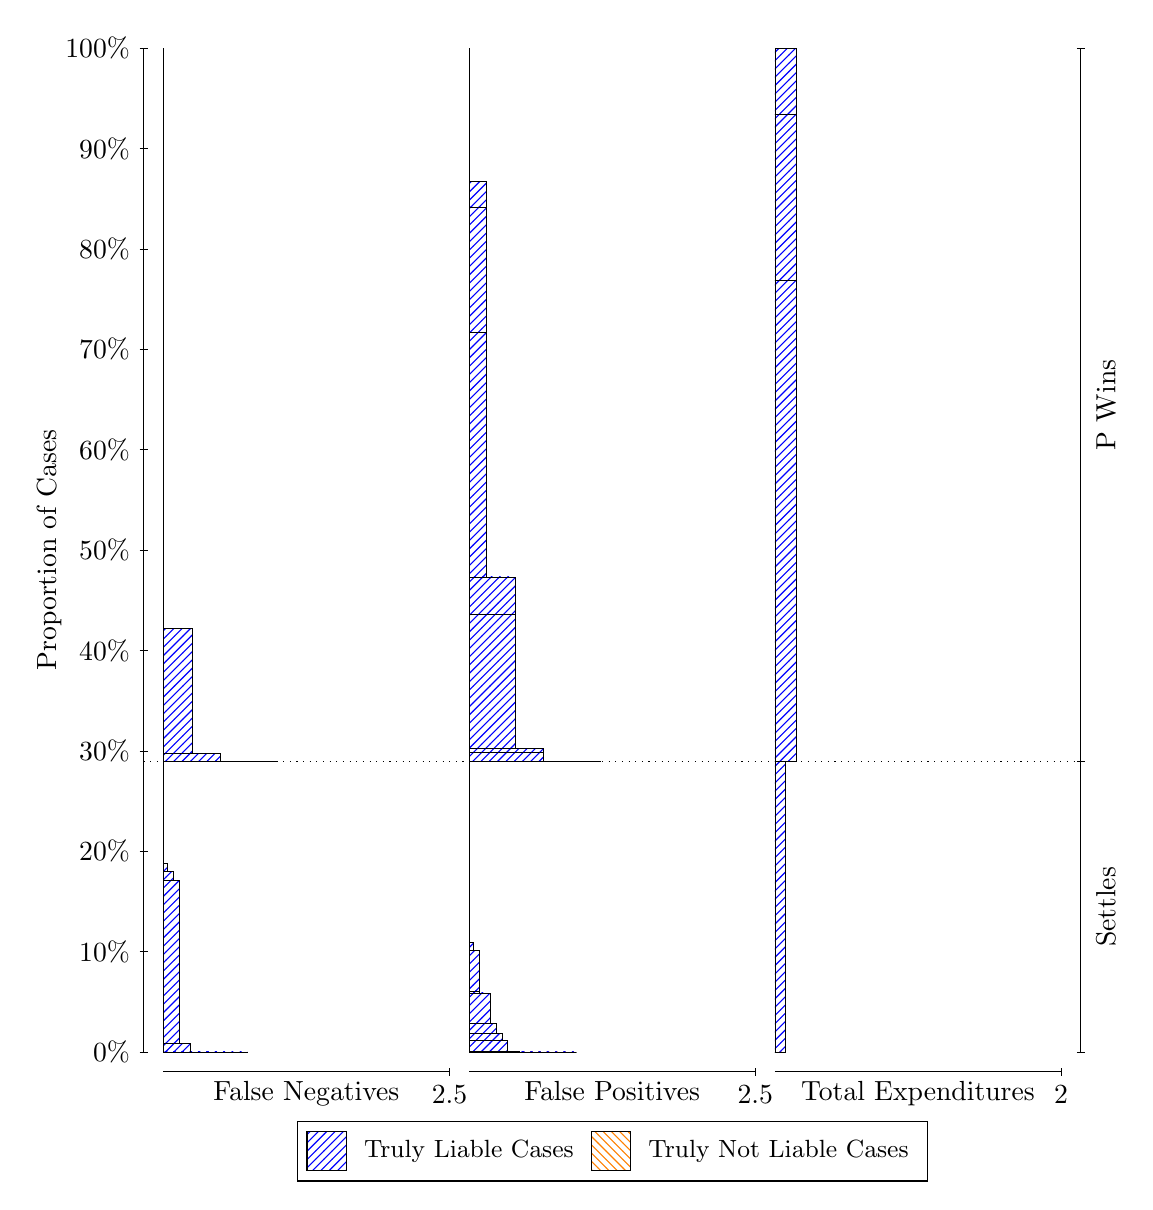
\begin{tikzpicture}
\draw[black, very thin] (1.5,1.75) -- (1.5,14.5);
\node[rotate=90, text=black, anchor=center] at (0.3, 8.125) {Proportion of Cases};
\draw[black, very thin] (1.45,1.75) -- (1.55,1.75);
\node[text=black, anchor=east] at (1.45, 1.75) {0\%};
\draw[black, very thin] (1.45,3.025) -- (1.55,3.025);
\node[text=black, anchor=east] at (1.45, 3.025) {10\%};
\draw[black, very thin] (1.45,4.3) -- (1.55,4.3);
\node[text=black, anchor=east] at (1.45, 4.3) {20\%};
\draw[black, very thin] (1.45,5.575) -- (1.55,5.575);
\node[text=black, anchor=east] at (1.45, 5.575) {30\%};
\draw[black, very thin] (1.45,6.85) -- (1.55,6.85);
\node[text=black, anchor=east] at (1.45, 6.85) {40\%};
\draw[black, very thin] (1.45,8.125) -- (1.55,8.125);
\node[text=black, anchor=east] at (1.45, 8.125) {50\%};
\draw[black, very thin] (1.45,9.4) -- (1.55,9.4);
\node[text=black, anchor=east] at (1.45, 9.4) {60\%};
\draw[black, very thin] (1.45,10.675) -- (1.55,10.675);
\node[text=black, anchor=east] at (1.45, 10.675) {70\%};
\draw[black, very thin] (1.45,11.95) -- (1.55,11.95);
\node[text=black, anchor=east] at (1.45, 11.95) {80\%};
\draw[black, very thin] (1.45,13.225) -- (1.55,13.225);
\node[text=black, anchor=east] at (1.45, 13.225) {90\%};
\draw[black, very thin] (1.45,14.5) -- (1.55,14.5);
\node[text=black, anchor=east] at (1.45, 14.5) {100\%};

\draw[black, very thin] (13.4,1.75) -- (13.4,14.5);
\draw[black, very thin] (13.35,1.75) -- (13.45,1.75);
\node[anchor=west] at (13.35, 1.75) {};
\draw[black, very thin] (13.35,5.4357) -- (13.45,5.4357);
\node[anchor=west] at (13.35, 5.4357) {};
\draw[black, very thin] (13.35,14.5) -- (13.45,14.5);
\node[anchor=west] at (13.35, 14.5) {};

\draw[black, very thin, pattern color=blue, pattern=north east lines] (1.75,1.75) rectangle (2.8218,1.75);
\draw[black, very thin, pattern color=blue, pattern=north east lines] (1.75,1.75) rectangle (2.5312,1.75);
\draw[black, very thin, pattern color=blue, pattern=north east lines] (1.75,1.75) rectangle (2.4585,1.7505);
\draw[black, very thin, pattern color=blue, pattern=north east lines] (1.75,1.7505) rectangle (2.3858,1.7505);
\draw[black, very thin, pattern color=blue, pattern=north east lines] (1.75,1.7505) rectangle (2.2405,1.7508);
\draw[black, very thin, pattern color=blue, pattern=north east lines] (1.75,1.7508) rectangle (2.1678,1.7516);
\draw[black, very thin, pattern color=blue, pattern=north east lines] (1.75,1.7516) rectangle (2.0952,1.8578);
\draw[black, very thin, pattern color=blue, pattern=north east lines] (1.75,1.8578) rectangle (2.0952,1.8593);
\draw[black, very thin, pattern color=blue, pattern=north east lines] (1.75,1.8593) rectangle (2.0225,1.8598);
\draw[black, very thin, pattern color=blue, pattern=north east lines] (1.75,1.8598) rectangle (1.9498,3.9274);
\draw[black, very thin, pattern color=blue, pattern=north east lines] (1.75,3.9274) rectangle (1.8772,4.0456);
\draw[black, very thin, pattern color=blue, pattern=north east lines] (1.75,4.0456) rectangle (1.8045,4.1427);
\draw[black, very thin, pattern color=orange, pattern=north west lines] (1.75,4.1427) rectangle (1.75,4.1427);
\draw[black, very thin, pattern color=blue, pattern=north east lines] (1.75,4.1427) rectangle (1.75,5.4357);
\draw[black, very thin, pattern color=blue, pattern=north east lines] (1.75,5.4357) rectangle (3.2033,5.4357);
\draw[black, very thin, pattern color=blue, pattern=north east lines] (1.75,5.4357) rectangle (2.84,5.4369);
\draw[black, very thin, pattern color=blue, pattern=north east lines] (1.75,5.4369) rectangle (2.4767,5.5469);
\draw[black, very thin, pattern color=blue, pattern=north east lines] (1.75,5.5469) rectangle (2.1133,7.1342);
\draw[black, very thin, pattern color=orange, pattern=north west lines] (1.75,7.1342) rectangle (1.75,7.1342);
\draw[black, very thin, pattern color=blue, pattern=north east lines] (1.75,7.1342) rectangle (1.75,14.5);
\draw[black, very thin, pattern color=orange, pattern=north west lines] (5.6333,1.75) rectangle (6.9958,1.75);
\draw[black, very thin, pattern color=blue, pattern=north east lines] (5.6333,1.75) rectangle (6.9958,1.75);
\draw[black, very thin, pattern color=orange, pattern=north west lines] (5.6333,1.75) rectangle (6.8505,1.75);
\draw[black, very thin, pattern color=blue, pattern=north east lines] (5.6333,1.75) rectangle (6.8505,1.75);
\draw[black, very thin, pattern color=orange, pattern=north west lines] (5.6333,1.75) rectangle (6.7052,1.75);
\draw[black, very thin, pattern color=blue, pattern=north east lines] (5.6333,1.75) rectangle (6.7052,1.75);
\draw[black, very thin, pattern color=blue, pattern=north east lines] (5.6333,1.75) rectangle (6.6325,1.75);
\draw[black, very thin, pattern color=orange, pattern=north west lines] (5.6333,1.75) rectangle (6.5598,1.75);
\draw[black, very thin, pattern color=blue, pattern=north east lines] (5.6333,1.75) rectangle (6.5598,1.75);
\draw[black, very thin, pattern color=blue, pattern=north east lines] (5.6333,1.75) rectangle (6.4872,1.75);
\draw[black, very thin, pattern color=orange, pattern=north west lines] (5.6333,1.75) rectangle (6.4145,1.75);
\draw[black, very thin, pattern color=blue, pattern=north east lines] (5.6333,1.75) rectangle (6.4145,1.7512);
\draw[black, very thin, pattern color=blue, pattern=north east lines] (5.6333,1.7512) rectangle (6.3418,1.7518);
\draw[black, very thin, pattern color=blue, pattern=north east lines] (5.6333,1.7518) rectangle (6.2692,1.7539);
\draw[black, very thin, pattern color=blue, pattern=north east lines] (5.6333,1.7539) rectangle (6.1965,1.7543);
\draw[black, very thin, pattern color=blue, pattern=north east lines] (5.6333,1.7543) rectangle (6.1238,1.7554);
\draw[black, very thin, pattern color=orange, pattern=north west lines] (5.6333,1.7554) rectangle (6.1238,1.7554);
\draw[black, very thin, pattern color=blue, pattern=north east lines] (5.6333,1.7554) rectangle (6.1238,1.8925);
\draw[black, very thin, pattern color=blue, pattern=north east lines] (5.6333,1.8925) rectangle (6.0512,1.9899);
\draw[black, very thin, pattern color=blue, pattern=north east lines] (5.6333,1.9899) rectangle (5.9785,2.1165);
\draw[black, very thin, pattern color=blue, pattern=north east lines] (5.6333,2.1165) rectangle (5.9058,2.4907);
\draw[black, very thin, pattern color=blue, pattern=north east lines] (5.6333,2.4907) rectangle (5.8332,2.4999);
\draw[black, very thin, pattern color=blue, pattern=north east lines] (5.6333,2.4999) rectangle (5.7605,2.5271);
\draw[black, very thin, pattern color=blue, pattern=north east lines] (5.6333,2.5271) rectangle (5.7605,3.043);
\draw[black, very thin, pattern color=blue, pattern=north east lines] (5.6333,3.043) rectangle (5.6878,3.1401);
\draw[black, very thin, pattern color=blue, pattern=north east lines] (5.6333,3.1401) rectangle (5.6333,5.4357);
\draw[black, very thin, pattern color=orange, pattern=north west lines] (5.6333,5.4357) rectangle (7.3047,5.4357);
\draw[black, very thin, pattern color=blue, pattern=north east lines] (5.6333,5.4357) rectangle (7.3047,5.4357);
\draw[black, very thin, pattern color=orange, pattern=north west lines] (5.6333,5.4357) rectangle (6.9413,5.4357);
\draw[black, very thin, pattern color=blue, pattern=north east lines] (5.6333,5.4357) rectangle (6.9413,5.4371);
\draw[black, very thin, pattern color=blue, pattern=north east lines] (5.6333,5.4371) rectangle (6.9413,5.4379);
\draw[black, very thin, pattern color=orange, pattern=north west lines] (5.6333,5.4379) rectangle (6.578,5.4379);
\draw[black, very thin, pattern color=blue, pattern=north east lines] (5.6333,5.4379) rectangle (6.578,5.5542);
\draw[black, very thin, pattern color=blue, pattern=north east lines] (5.6333,5.5542) rectangle (6.578,5.6035);
\draw[black, very thin, pattern color=orange, pattern=north west lines] (5.6333,5.6035) rectangle (6.2147,5.6035);
\draw[black, very thin, pattern color=blue, pattern=north east lines] (5.6333,5.6035) rectangle (6.2147,7.3074);
\draw[black, very thin, pattern color=blue, pattern=north east lines] (5.6333,7.3074) rectangle (6.2147,7.7843);
\draw[black, very thin, pattern color=blue, pattern=north east lines] (5.6333,7.7843) rectangle (5.8513,10.886);
\draw[black, very thin, pattern color=orange, pattern=north west lines] (5.6333,10.886) rectangle (5.8513,10.886);
\draw[black, very thin, pattern color=blue, pattern=north east lines] (5.6333,10.886) rectangle (5.8513,12.483);
\draw[black, very thin, pattern color=blue, pattern=north east lines] (5.6333,12.483) rectangle (5.8513,12.802);
\draw[black, very thin, pattern color=blue, pattern=north east lines] (5.6333,12.802) rectangle (5.6333,14.5);
\draw[black, very thin, pattern color=orange, pattern=north west lines] (9.5167,1.75) rectangle (9.6529,1.75);
\draw[black, very thin, pattern color=blue, pattern=north east lines] (9.5167,1.75) rectangle (9.6529,5.4357);
\draw[black, very thin, pattern color=orange, pattern=north west lines] (9.5167,5.4357) rectangle (9.7892,5.4357);
\draw[black, very thin, pattern color=blue, pattern=north east lines] (9.5167,5.4357) rectangle (9.7892,11.552);
\draw[black, very thin, pattern color=orange, pattern=north west lines] (9.5167,11.552) rectangle (9.7892,11.552);
\draw[black, very thin, pattern color=blue, pattern=north east lines] (9.5167,11.552) rectangle (9.7892,13.655);
\draw[black, very thin, pattern color=orange, pattern=north west lines] (9.5167,13.655) rectangle (9.7892,13.655);
\draw[black, very thin, pattern color=blue, pattern=north east lines] (9.5167,13.655) rectangle (9.7892,14.5);
\draw[black, dotted] (1.5,5.4357) -- (13.4,5.4357);
\draw[black, very thin] (1.75,1.5) -- (5.3833,1.5);
\node[text=black, anchor=north] at (3.5667, 1.5) {False Negatives};
\draw[black, very thin] (5.3833,1.45) -- (5.3833,1.55);
\node[text=black, anchor=north] at (5.3833, 1.45) {2.5};

\draw[black, very thin] (5.6333,1.5) -- (9.2667,1.5);
\node[text=black, anchor=north] at (7.45, 1.5) {False Positives};
\draw[black, very thin] (9.2667,1.45) -- (9.2667,1.55);
\node[text=black, anchor=north] at (9.2667, 1.45) {2.5};

\draw[black, very thin] (9.5167,1.5) -- (13.15,1.5);
\node[text=black, anchor=north] at (11.333, 1.5) {Total Expenditures};
\draw[black, very thin] (13.15,1.45) -- (13.15,1.55);
\node[text=black, anchor=north] at (13.15, 1.45) {2};

\node[text=black, centered, rotate=90] at (13.72, 3.5929) {Settles};
\node[text=black, centered, rotate=90] at (13.72, 9.9679) {P Wins};

\draw (7.449999999999999,1.5) node[draw=none] (baseCoordinate) {};
\begin{scope}[align=center]
        \matrix[scale=0.5, draw=black, below=0.5cm of baseCoordinate, nodes={draw}, column sep=0.1cm]{
            \node[rectangle, draw, minimum width=0.5cm, minimum height=0.5cm, pattern color=blue, pattern=north east lines] {}; &
            \node[draw=none, font=\small, text=black] (B) {Truly Liable Cases}; &
            \node[rectangle, draw, minimum width=0.5cm, minimum height=0.5cm, pattern color=orange, pattern=north west lines] {}; &
            \node[draw=none, font=\small, text=black] (B) {Truly Not Liable Cases}; \\
            };
\end{scope}

\end{tikzpicture}
\end{document}